\documentclass{beamer}

\usepackage[utf8]{inputenc}
%\usepackage{adjustbox}
\usepackage[export]{adjustbox}
\usepackage{booktabs}
%\usepackage{ctex}
\usepackage{graphicx}
\usepackage{subcaption}

\captionsetup{compatibility=false}

\graphicspath{ {images/} }

\usetheme{Madrid}

\title[OJ user behavior]{The User Behavior On Online Judge Website }
\author[yiyuezhuo]{yueyi zhuo}
\institute[SICNU]{School of Mathematical,Sichuan Normal University}
\date{2017}

\begin{document}

\frame{\titlepage}

\begin{frame}

\frametitle{What is online judge(OJ)?}

An online judge is an online system to test programs in programming contests. 
They are also used to practice for such contests. Many of these systems organize their own contests.

The system can compile and execute code, and test them with pre-constructed data. 
Submitted code may be run with restrictions, including time limit, memory limit, security restriction and so on. 
The output of the code will be captured by the system, and compared with the standard output. 
The system will then return the result. When mistakes were found in a standard output, 
rejudgement using the same method must be made.

Online Judges have ranklists showing users with the biggest number of accepted solutions and shortest 
execution time for a particular problem. \footnote{Wikipedia https://en.wikipedia.org/wiki/Online\_judge}

\end{frame}

\begin{frame}
\frametitle{Project Euler}
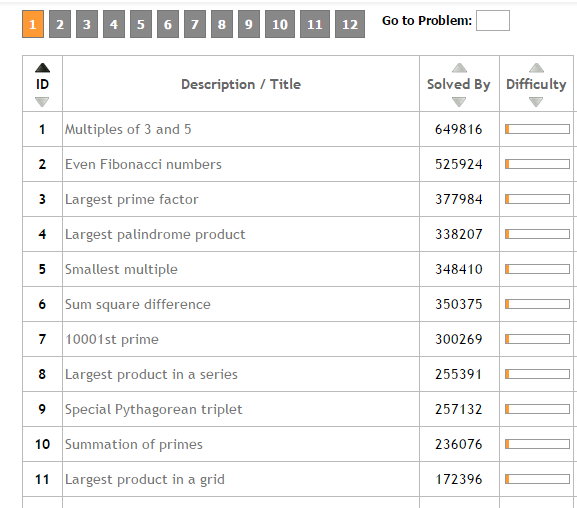
\includegraphics[scale=0.55]{euler-oj.png}
\end{frame}

\begin{frame}
\frametitle{leetcode OJ}
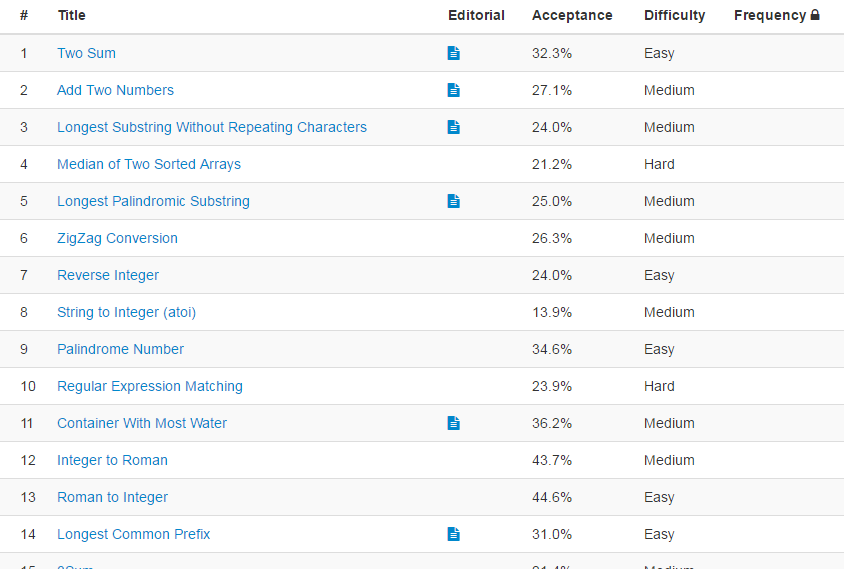
\includegraphics[scale=0.4]{leetcode-oj.png}
\end{frame}


\begin{frame}
\frametitle{Sicnu OJ}
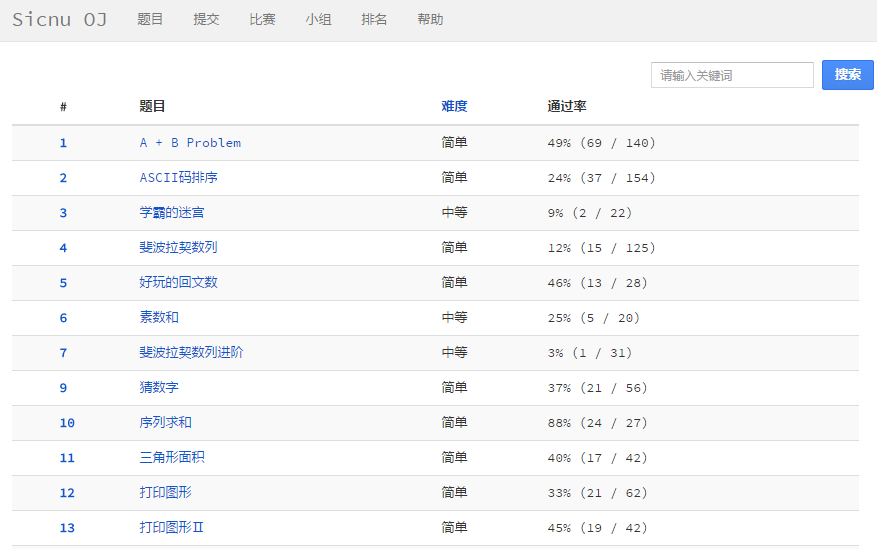
\includegraphics[scale=0.5]{sicnu-oj.png}
\end{frame}

\begin{frame}
\frametitle{Some problem in Real world}

The data listed on the table looks very interesting. These're a number of insights for user behavior which 
can generalize to online education service. For example:

Why the sequence of number of solved looks like this? If we provide online education product as same as those oj, 
and observe such series, does it mean our product fail or extra-success?

\begin{figure}[h]
 
\begin{subfigure}{0.45\textwidth}
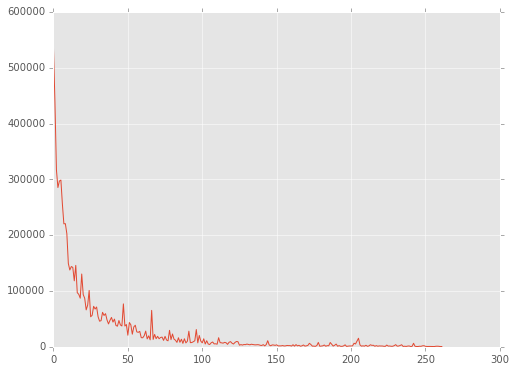
\includegraphics[width=0.9\linewidth, height=4cm]{solved-seq1.png} 
\caption{Solved number series}
\label{fig:f1}
\end{subfigure}
\begin{subfigure}{0.45\textwidth}
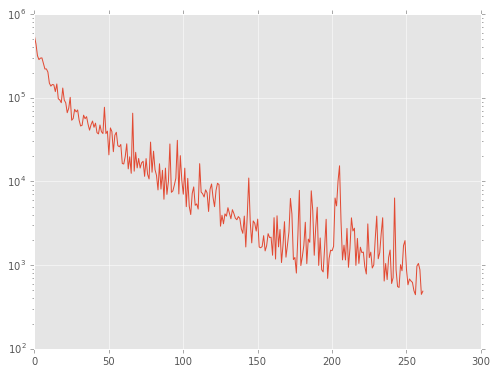
\includegraphics[width=0.9\linewidth, height=4cm]{solved-seq2.png}
\caption{Log solved number series}
\label{fig:f2}
\end{subfigure}
 
\caption{Caption for this figure with two images}
\label{fig:image2}
\end{figure}

\end{frame}

\begin{frame}

\frametitle{Identify}

Is it signicant to put difficult problem on the behind those easy problem 
if we want keep our user satisfactory and not be shocked by excess hard problem? It make sense
for online education to maintain user interest in their study process. For technically speaking:
According to data, do we observe the fact that a hard problem cause a temporary 
or continued solved number decrease, although we have controlled other effect? 

How do we control other effect to identify the shock from hard problem? The econometric model might help, 
following regression models have been run as baseline to lead to thee problem that we try to survey.

\end{frame}

\begin{frame}

\frametitle{Model 1}

$$
solve_i = \beta_0 + \beta_1 id_i + \beta_2 diff_i + \epsilon_i
$$

where $id_i$ is the id of problem $i$, $diff_i$ is difficulty measure given by Project Euler.

\begin{center}
\scalebox{0.5}[0.5]{
\begin{tabular}{lclc}
\toprule
\textbf{Dep. Variable:}    &      solve       & \textbf{  R-squared:         } &    0.331  \\
\textbf{Model:}            &       OLS        & \textbf{  Adj. R-squared:    } &    0.325  \\
\textbf{Method:}           &  Least Squares   & \textbf{  F-statistic:       } &    63.95  \\
\textbf{Date:}             & Mon, 10 Apr 2017 & \textbf{  Prob (F-statistic):} & 2.68e-23  \\
\textbf{Time:}             &     22:53:04     & \textbf{  Log-Likelihood:    } &  -3224.6  \\
\textbf{No. Observations:} &         262      & \textbf{  AIC:               } &    6455.  \\
\textbf{Df Residuals:}     &         259      & \textbf{  BIC:               } &    6466.  \\
\textbf{Df Model:}         &           2      & \textbf{                     } &           \\
\textbf{Covariance Type:}  &    nonrobust     & \textbf{                     } &           \\
\bottomrule
\end{tabular}
%\caption{OLS Regression Results}
}
\scalebox{0.5}[0.5]{
\begin{tabular}{lccccc}
\toprule
                   & \textbf{coef} & \textbf{std err} & \textbf{t} & \textbf{P$>$$|$t$|$} & \textbf{[95.0\% Conf. Int.]}  \\
\midrule
\textbf{Intercept} &    9.401e+04  &     6678.292     &    14.077  &         0.000        &      8.09e+04  1.07e+05       \\
\textbf{id}        &    -479.7585  &       90.521     &    -5.300  &         0.000        &      -658.008  -301.509       \\
\textbf{diff}      &     -60.2227  &      266.704     &    -0.226  &         0.822        &      -585.406   464.961       \\
\bottomrule
\end{tabular}
}
\scalebox{0.5}[0.5]{
\begin{tabular}{lclc}
\toprule
\textbf{Omnibus:}       & 270.575 & \textbf{  Durbin-Watson:     } &    0.077  \\
\textbf{Prob(Omnibus):} &   0.000 & \textbf{  Jarque-Bera (JB):  } & 8178.806  \\
\textbf{Skew:}          &   4.299 & \textbf{  Prob(JB):          } &     0.00  \\
\textbf{Kurtosis:}      &  28.986 & \textbf{  Cond. No.          } &     317.  \\
\bottomrule
\end{tabular}
}
\end{center}

\end{frame}

\begin{frame}

We can see the estimated effect of $diff$ is negative but not be signicant. 
While the result does not adapt for theory,
DW statistic is too low which imply possibility that autocorrelation exist in model. 
Let we try to apply log transform on $solve$ to reduce the effect and to make estimated value more precise.

\begin{figure}[h]
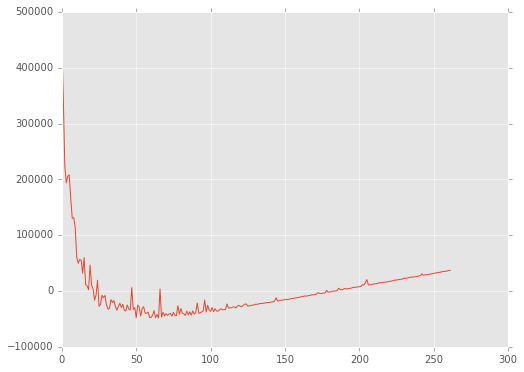
\includegraphics[width=0.5\textwidth, inner]{model1-resid.png}
\caption{Plot of residuals of model 1}
\label{fig:f3}
\end{figure}

\end{frame}

\begin{frame}

\frametitle{Model 2}


The only change of model 2 is that dependent variable $solve$ is transform to $log(solve)$.
$$
\log(solve_i) = \beta_0 + \beta_1 id_i + \beta_2 diff_i + \epsilon_i
$$

\begin{center}
\scalebox{0.5}[0.5]{
\begin{tabular}{lclc}
\toprule
\textbf{Dep. Variable:}    &    log(solve)    & \textbf{  R-squared:         } &     0.943  \\
\textbf{Model:}            &       OLS        & \textbf{  Adj. R-squared:    } &     0.943  \\
\textbf{Method:}           &  Least Squares   & \textbf{  F-statistic:       } &     2150.  \\
\textbf{Date:}             & Mon, 10 Apr 2017 & \textbf{  Prob (F-statistic):} & 4.94e-162  \\
\textbf{Time:}             &     23:27:00     & \textbf{  Log-Likelihood:    } &   -128.21  \\
\textbf{No. Observations:} &         262      & \textbf{  AIC:               } &     262.4  \\
\textbf{Df Residuals:}     &         259      & \textbf{  BIC:               } &     273.1  \\
\textbf{Df Model:}         &           2      & \textbf{                     } &            \\
\textbf{Covariance Type:}  &    nonrobust     & \textbf{                     } &            \\
\bottomrule
\end{tabular}
%\caption{OLS Regression Results}
}
\scalebox{0.5}[0.5]{
\begin{tabular}{lccccc}
\toprule
                   & \textbf{coef} & \textbf{std err} & \textbf{t} & \textbf{P$>$$|$t$|$} & \textbf{[95.0\% Conf. Int.]}  \\
\midrule
\textbf{Intercept} &      11.4369  &        0.049     &   232.406  &         0.000        &        11.340    11.534       \\
\textbf{id}        &      -0.0081  &        0.001     &   -12.179  &         0.000        &        -0.009    -0.007       \\
\textbf{diff}      &      -0.0407  &        0.002     &   -20.685  &         0.000        &        -0.045    -0.037       \\
\bottomrule
\end{tabular}
}
\scalebox{0.5}[0.5]{
\begin{tabular}{lclc}
\toprule
\textbf{Omnibus:}       & 117.312 & \textbf{  Durbin-Watson:     } &     0.197  \\
\textbf{Prob(Omnibus):} &   0.000 & \textbf{  Jarque-Bera (JB):  } &   466.808  \\
\textbf{Skew:}          &   1.888 & \textbf{  Prob(JB):          } & 4.30e-102  \\
\textbf{Kurtosis:}      &   8.339 & \textbf{  Cond. No.          } &      317.  \\
\bottomrule
\end{tabular}
}
\end{center}

\end{frame}

\begin{frame}

New model make $diff$ significant but DW statistic still be too small (0.197 from 0.07). 
Since $diff$ is not a real quantity index which take value as 5, 10, etc for no reason,
we replace it to two new dummy variables $diff\_mid$ and $diff\_hard$. 
$diff\_mid_i=1$ if $diff > 25$,else $diff\_mid_i=0$.
$diff\_hard_i=1$ if $diff > 50$,else $diff\_hard_i=0$.


\begin{figure}[h]
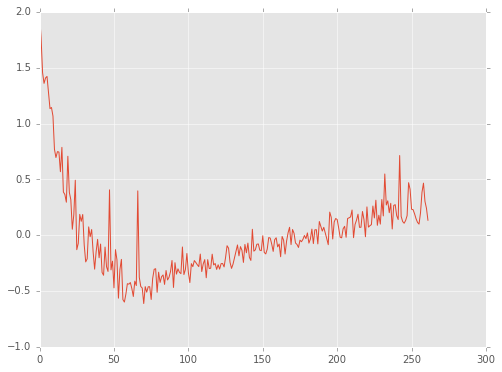
\includegraphics[width=0.5\textwidth, inner]{model2-resid.png}
\caption{Plot of residuals of model 2}
\label{fig:f4}
\end{figure}

\end{frame}

\begin{frame}

\frametitle{Model 3}

$$
\log(solve_i) = \beta_0 + \beta_1 id_i + \beta_2 diff\_mid + \beta_3 diff\_hard + \epsilon_i
$$

\begin{center}
\scalebox{0.5}[0.5]{
\begin{tabular}{lclc}
\toprule
\textbf{Dep. Variable:}    &    log(solve)    & \textbf{  R-squared:         } &     0.907  \\
\textbf{Model:}            &       OLS        & \textbf{  Adj. R-squared:    } &     0.906  \\
\textbf{Method:}           &  Least Squares   & \textbf{  F-statistic:       } &     841.8  \\
\textbf{Date:}             & Tue, 11 Apr 2017 & \textbf{  Prob (F-statistic):} & 6.87e-133  \\
\textbf{Time:}             &     14:38:30     & \textbf{  Log-Likelihood:    } &   -192.36  \\
\textbf{No. Observations:} &         262      & \textbf{  AIC:               } &     392.7  \\
\textbf{Df Residuals:}     &         258      & \textbf{  BIC:               } &     407.0  \\
\textbf{Df Model:}         &           3      & \textbf{                     } &            \\
\textbf{Covariance Type:}  &    nonrobust     & \textbf{                     } &            \\
\bottomrule
\end{tabular}
%\caption{OLS Regression Results}
}
\scalebox{0.5}[0.5]{
\begin{tabular}{lccccc}
\toprule
                           & \textbf{coef} & \textbf{std err} & \textbf{t} & \textbf{P$>$$|$t$|$} & \textbf{[95.0\% Conf. Int.]}  \\
\midrule
\textbf{Intercept}         &      11.2770  &        0.066     &   169.869  &         0.000        &        11.146    11.408       \\
\textbf{diff\_mid[T.True]}  &      -1.0259  &        0.102     &   -10.088  &         0.000        &        -1.226    -0.826       \\
\textbf{diff\_hard[T.True]} &      -0.6194  &        0.092     &    -6.731  &         0.000        &        -0.801    -0.438       \\
\textbf{id}                &      -0.0124  &        0.001     &   -16.695  &         0.000        &        -0.014    -0.011       \\
\bottomrule
\end{tabular}
}
\scalebox{0.5}[0.5]{
\begin{tabular}{lclc}
\toprule
\textbf{Omnibus:}       & 32.712 & \textbf{  Durbin-Watson:     } &    0.774  \\
\textbf{Prob(Omnibus):} &  0.000 & \textbf{  Jarque-Bera (JB):  } &   45.065  \\
\textbf{Skew:}          &  0.810 & \textbf{  Prob(JB):          } & 1.64e-10  \\
\textbf{Kurtosis:}      &  4.225 & \textbf{  Cond. No.          } &     501.  \\
\bottomrule
\end{tabular}
}
\end{center}

\end{frame}

\begin{frame}

The DW statistic looks better than using $diff$ directly. But if we inspect the the plot of residual of model3, 
the same pattern is weaken while there aren't fundamentally changed to what we expect.

\begin{figure}[h]
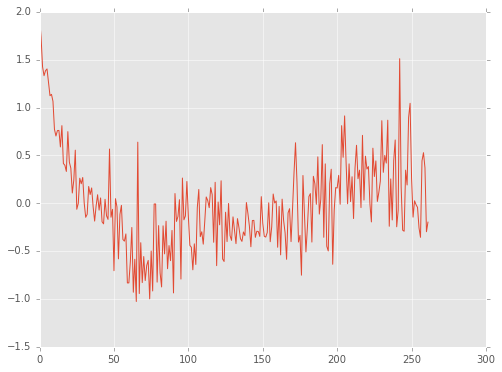
\includegraphics[width=0.5\textwidth, inner]{model3-resid.png}
\caption{Plot of residuals of model 3}
\end{figure}

\end{frame}

\begin{frame}

\frametitle{What construct the residual pattern? The road to user personas. }

Although we can run a segmented regression, but more fundamental origin is interesting to investigate.
A idea to model this phenomenon is to try to decompose user into distinct groups
who acts differently in problem solving process. 

For example, the "light" user may solve first few problems and then leave while the "hard core" 
user would try solve many problem until their interest wore off and nerd would like to solve prolbem
labeled as hardest. 

How to esimate these latent factor? The solved sequence may be too weak to apply identification. 
Fortunately, some extra-date have been collected for the goal.

%These effects are mixed and hard to distinguish if we only consider the infomation given by OJ website.

%For example, the number of hit of chinese translation of description of origin problem is a variable relate 
%solved number. In fact, we can run a parallel model on hit data.

\end{frame}

\begin{frame}

\frametitle{Extended Data Structure and Cross Estimation}

These's a chinese translation website that provide problem description translation for original problem.
Obviously, the hit count of problem is a important factor to measure problem real difficulty taken by to compare 
hit and solved number. Sadly, Project Euler dont't provide this measure directly, 
but the hit prodived by translation post would be a nice proxy variable. Of course the method cause new problem.
Someone may looks chinese translation post for their poor English(like me), 
thus if we equally weight eveny posts, then the problem hard to read will be exaggerated on their difficulty estimated.
Against this challenge, I collect the text length of description in both English(origin) and Chinese(translation) version,
although the difficulty in readability but not problem may be caused by some vague statement or confusing grammar
that can't be caught by text length.


\end{frame}

\begin{frame}

If we assume that these OJ shares same user and their behavior distribution, 
we can estimate these hidden parameters on a more horizon space, instead of only to observe one sequence 
as the only one sample to model, and use data only not hold in one OJ but hold in other. For example, 
as previous images, Project Euler doesn't include Acceptance index, but the two others does, hence we can use the two
others index to fill Project Euler one. How excellent idea! Thanks internet prodive so many website which 
provide same and distinct index from their "nature experiment". Big data equip us with these advanced tool
to investigate world that hided in past.

The current data structure looks like this:

\begin{tabular}{lrrrrrrr}
\toprule
{} &  id &  content &  des\_len &  diff &    hit &   solve &  t\_content \\
\midrule
0 &   1 &      187 &       25 &     5 &  13792 &  537234 &         85 \\
1 &   2 &      312 &       32 &     5 &   7571 &  438350 &        135 \\
2 &   3 &      111 &       17 &     5 &   6364 &  317208 &         65 \\
3 &   4 &      209 &       20 &     5 &   5414 &  285419 &        101 \\
4 &   5 &      206 &       24 &     5 &   4627 &  297082 &         70 \\
\bottomrule
\end{tabular}

\end{frame}

\begin{frame}

\frametitle{The Power of Cross Estimation, A Example}

Let's see a example about the power in cross estimation. The following is hit sequence, what made the abrupt decrease?
Compare to original sequence, we can't see same pattern. For any reason, these's a change to run regression discontinuity
to identify some effect that are hard to identify usually.

\begin{figure}[h]
 
\begin{subfigure}{0.45\textwidth}
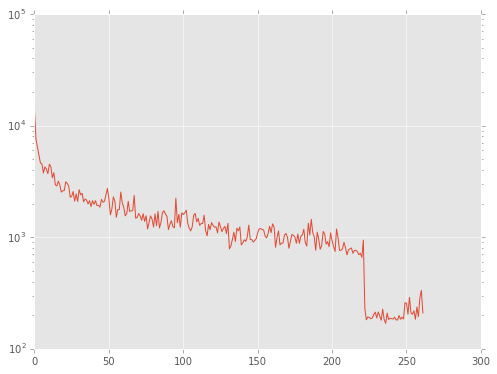
\includegraphics[width=0.9\linewidth, height=4cm]{hit-seq.png} 
\caption{Hit number series}
\label{fig:f1}
\end{subfigure}
\begin{subfigure}{0.45\textwidth}
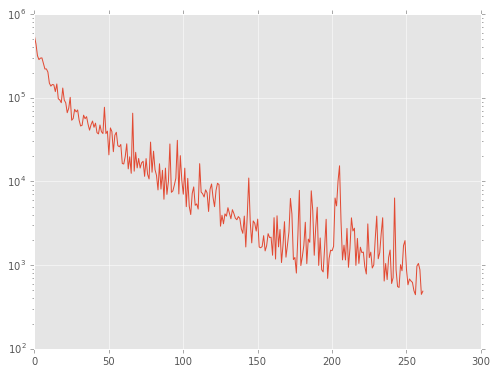
\includegraphics[width=0.9\linewidth, height=4cm]{solved-seq2.png}
\caption{Log solved number series}
\label{fig:f2}
\end{subfigure}
 
%\caption{Caption for this figure with two images}
\label{fig:image2}
\end{figure}


\end{frame}

\end{document}
